\subsection{Composition Concepts}

The major challenge during the development of a \ms{} application is to achieve
loose coupling according to the IDEAL tenet. The goal of loose coupling is to
reduce dependencies among services. It has to be noticed that the coupling
between services can never be zero. Without any coupling the application cannot
function as a whole. MicroNet follows three basic concepts to reduce service
coupling while preserving reasonable development comfort.

\subsubsection{Dependency Abstraction}

Dependency abstraction is a concept to reduce the number of dependency
includes like for example the number of classpath entries of a Java application.

According to the dependency abstraction concept external libraries are wrapped
within a set of adapters which offer standard access to the underlying
dependency. Services can use this adapter instead of using the dependency
directly. This allows for exchangeability of the dependencies without touching
the services.

It has to be mentioned that the dependency abstraction layer is a dependency
itself and therefore it increases service coupling. But since the abstraction
layer unifies dependency access it helps to respect the don't repeat yourself (DRY)
principle and therefore increases overall cohesion of the application. 

In MicroNet the adaption layer is realized using Java wrapper libraries. For all
Java services this approach works very well but none Java services have to
either implement their own wrapper or use the dependencies natively. MicroNet
wrapper libraries are: Serialization, Networking, and Persistence.

\subsubsection{Shared Model}
\label{subsub:shared_model}

The general design of how to incorporate a game model \mn{} is reclined to the
design of modern game engines like Unity3D or UnrealEngine 4. What these engines
have in common is a graph to describe the game e.g. all objects, levels,
players, etc. which are part of the game. This concept of game data organization
will be referred as the game graph. Two examples of game graphs are shown in
\autoref{fig:scenegraph}.

\begin{figure}
  \centering
  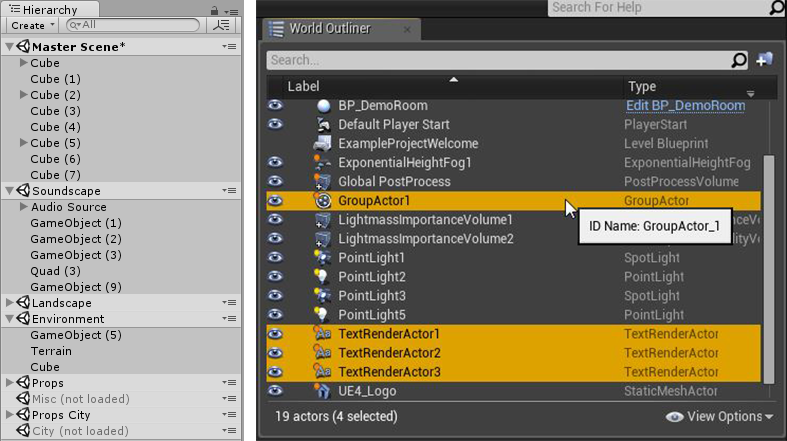
\includegraphics[width=\textwidth]{images/game_engine/scenegraph}
  \caption{Two example game graphs of the Unity3D (left) and the UnrealEngine4
  (right).}
  \label{fig:scenegraph}
\end{figure}

The shared model concept is mainly inspired by game graph concept of game
engines. The idea behind the model is to reduce coupling of \ms{} by sharing the
domain model of the game in the form of a game graph. This graph is defined in
Json format and can be shared either using a git repository or by using a
development database. The Json format helps to achieve platform independence.

The shared model allows to strongly type message transfers and unifies database
access. It also allows simple integration of the domain model in the game graph
of a game engine. \autoref{lst:template_type} shows an example of a template
type graph used by MicroNet.

\begin{figure}
	\begin{lstlisting}[language=json,firstnumber=1] 
	{
	  "name": "UserValues",
	  "variables": [
	    {
	      "name": "id",
	      "type": {
	        "numberType": "INT",
	        "type": "NUMBER"
	      }
	    },
	    {
	      "name": "credentials",
	      "type": {
	        "componentType": "CredentialValues",
	        "type": "COMPONENT"
	      }
	    }
	  ]
	}
	\end{lstlisting}
  	\caption{The model graph of the UserValues domain object.}
  	\label{lst:template_type}
\end{figure}

\subsubsection{Service API}

Two major challenge in distributed application development is service discovery
and message transfer semantics. To provide service discovery MicroNet defines
the Service API as static URIs in the form:
``ms://servicename/fine/grained/api''. The host portion of the URI is used for
participant discovery by using the message broker functionality to register
queues for the specific service address, ``ms://servicename'' in this example.
The remainder of the URI, ``fine/grained/api'' in this example represents the
fine grained service API according to tenet Fine-grained Interfaces. This
Service API scheme of MicroNet is based on a RESTful URI schema. The service API
is defined using Java annotations \todo{ref}.

\subsubsection{Service Catalogue}

The service catalogue is a layer of MicroNet that uses the underlying framework
to provide reference service implementation to commonly requires functionality.
The service catalogue is realized by using Maven archetypes. The archetypes
represent a skeleton or a basic implementation of a feature and can be extended
by the developer. Often used functionality can be contributed to the service
catalogue to make it available for future reuse.

The service catalogue also contains a ``Hello World'' service that can be used
to bring up a new \ms{} quickly.

\subsubsection{Consistency Requirements}

Consistency is a big concern in any distributed application and \ogs{} are no
exception. For \ogs{} consistency requirements can be categorized into strong
consistency for sensitive data like account or payment information and best
effort consistency for all other game data. This aspect has been highlighted in
project thesis two \todo{cite thesis 2}.

The final solution to consistency in MicroNet is a solution to emphasis
exactly this two requirements. For strong consistency it is aways necessary that
one single service can process a complete transaction. This service then can
make a transaction ACID by using the two phase commit protocol offered by the
database. MicroNet uses ProstgreSQL for this purpose.

For best effort consistency requirements eventual consistency is a solution that
is proven to work \cite{graham2016distributed_transactions}. Eventual
consistency emphasis scaling and robust systems in general. The drawback is the
added effort during development to implement a eventual consistent application.
